\documentclass{beamer}
\usepackage{ctex}
\usepackage[export]{adjustbox}
\usepackage{listings}
\usepackage{xcolor}

\usetheme{focus}

\definecolor{codegreen}{RGB}{50 200 50}
\definecolor{codeblue}{RGB}{50 50 200}
\definecolor{codered}{RGB}{200 50 50}
\tikzset{
    global scale/.style={scale=#1,every node/.append style={scale=#1}},
    CC1/.style ={circle,minimum width = 30pt, minimum height =30pt, draw=black},
    CC2/.style ={circle,minimum width = 30pt, minimum height =30pt, draw=black, fill=blue!20},
    RA1/.style ={rectangle,minimum width = 30pt, minimum height =20pt, draw=black},
    RA2/.style ={rectangle,minimum width = 1cm, minimum height = 1cm, draw=black}
}

\title{算法分析与设计II}
\subtitle{2022-2023-2}
\date{Last Modified: 2023.1.16}
\institute{\vspace{2em} 数学与计算机学院 \\ 数据科学与大数据技术}
\titlegraphic{\vspace{5em} 
\includegraphics[scale=0.3]{fig/jlnu.pdf}}

\lstset{
    columns=flexible,       
    numbers=left,  
    numberstyle=\footnotesize\color{darkgray},  
    frame=shadowbox, 
    rulesepcolor= \color{gray}, 
    keywordstyle=\color{codeblue},         
    commentstyle=\color{codegreen},  
    stringstyle=\color{codered}, 
    showstringspaces=false,  
    xleftmargin=3em,
    xrightmargin=1em,              
    language=c++                           
}

\tikzset{
    CC1/.style ={
    circle,
    minimum width = 30pt, 
    minimum height =30pt, 
    draw=black
    }
}

\begin{document}
\frame{\titlepage}
\section{8. 图算法}
\begin{frame}{8.1 最小生成树}
    \begin{itemize}
        \item \textcolor{blue}{最小生成树}(MST, Minimum spanning tree)通常是在无向图问题中, 给出端点和两点之间边的权值,然后进行求解
        \item 图的存储给出邻接矩阵,转化为用边的存储结构来表示
        \item 常用的两种算法都是基于贪心策略
        \begin{itemize}
            \item \textcolor{blue}{Prim算法},利用最小堆来实现,运行时间取决于最小堆的实现方式
            \item \textcolor{blue}{Kruskal算法},需要将边按权值排序依次进行比较,当边较多时,运行时间会增加
        \end{itemize}
    \end{itemize}
\end{frame}
\begin{frame}{1258 -- Agri-Net (poj.org)}
    \begin{itemize}
        \item 有$n$个农场,给出相互之间的距离,用光纤将所有农场连接在一起,问如何连接使光纤总长度最小,求出这个最小值。即在$n$个点,$\frac {n(n-1)}{2}$条边组成的连通加权无向图中求最小生成树,本题使用Prim算法
    \end{itemize}
    \begin{block}{Prim算法}
        \quad 使用的是贪心策略,从单一顶点开始,依次加入其他顶点,保证加入的边长度最小,直到包含所有顶点结束
    \end{block}
    \begin{itemize}
        \item 定义二维数组D[i,j]为i到j的距离,在图论中,这种图结构的表示方法叫做\textcolor{blue}{邻接矩阵}(adjacency matrix)
        \item 用结构体edge\{v,to\}来表示图中的边(v为边权,to为边的终点)
        \item 定义vis[i]记录i点是否已经加入生成树中
        \item 将边放入最小堆Q来实现存取
    \end{itemize}
\end{frame}
\begin{frame}{计算过程}
    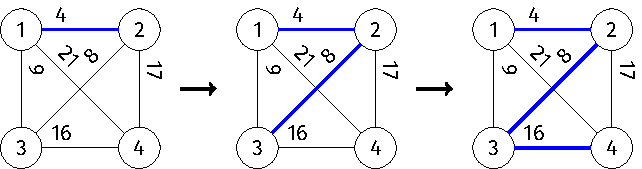
\includegraphics{fig/8-1.pdf}
\begin{enumerate}[(1)]
    \item 将顶点1加入生成树,设vis[1]=1,边\{4,2\},\{9,3\},\{21,4\}插入最小堆\pause
    \item 取出边\{4,2\},因为vis[2]=0,将2加入生成树,设vis[2]=1,累计距离等于4,边\{4,1\},\{8,3\},\{17,4\}插入最小堆\pause
    \item 取出边\{4,1\},因为vis[1]=1,继续;再取\{8,3\},因为vis[3]=0,将3加入生成树,设vis[3]=1,累计距离等于12,相应边插入最小堆\pause
    \item 依次取出边\{8,2\},\{9,1\},\{16,4\},因为vis[4]=0,将4加入生成树,设vis[4]=1,累计距离等于28,相应边插入最小堆\pause
    \item 继续从队列中取边,直到队列为空
\end{enumerate}
\end{frame}
\begin{frame}{2485 -- Highways (poj.org)}
    \begin{itemize}
        \item 给出$n$个城镇相互之间的距离,用高速公路连接所有城镇,求需要修建总长度最短的高速公路的方案中最长的一段公路的长度,本题使用Kruskal算法
    \end{itemize}    
    \begin{block}{Kruskal算法}
        使用的是贪心策略,将所有的边按长度递增排序,每次取一条边,如果没有形成回路, 就将这条边放入生成树中,直到检查完所有的边
    \end{block}
    \begin{itemize}
        \item 用结构体edge\{u,v,w\}来表示图中的边(u,v为边的两个端点,w为边的长度)
        \item 是否存在回路的判断,可以使用并查集来实现
    \end{itemize}
\end{frame}    
\begin{frame}{计算过程}
    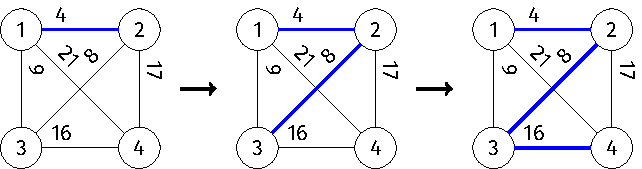
\includegraphics{fig/8-1.pdf}
\begin{enumerate}[(1)]
    \item 取\{1,2,4\},没有环路,将\{1,2,4\}放入生成树\pause
    \item 取\{2,3,8\},没有环路,将\{2,3,8\}放入生成树\pause
    \item 取\{1,3,9\},有环路,继续操作\pause
    \item 取\{3,4,16\},没有环路,将\{3,4,16\}放入生成树\pause
    \item 取\{2,4,17\},\{1,4,21\},有环路,继续操作\pause
    \item 所有边取完,过程结束,最后取的边\{3,4,16\}的长度就是本题的解
\end{enumerate}
\end{frame}
\begin{frame}{8.2 最短路}
    \begin{itemize}
        \item 在图中寻找两个节点之间的最短路径,称为\textcolor{blue}{最短路径问题} (Shortest path problem)
        \item 求最短路有以下几种常见的算法:
        \begin{itemize}
            \item 弗洛伊德(Floyd-Warshall)算法
            \item 贝尔曼-福特(Bellman-Ford)算法
            \item 最短路径快速算法(SPFA)
            \item 迪杰斯特拉(Dijkstra)算法
        \end{itemize}
    \end{itemize}
    \begin{table}
        \scriptsize{
        \begin{tabular}{l|l|l}
            \textbf{算法} & \textbf{代码中采用的数据结构} & \textbf{时间复杂度($V$:点数;$E$:边数)}\\\hline
			Floyd        & 邻接矩阵                 & $O(V^3)$    \\\hline
			Bellman-Ford & 邻接表                   & $O(VE)$     \\\hline
			SPFA         & 链式前向星               & 平均$O(2E)$,最差$O(VE)$  \\\hline
			Dijkstra     & 邻接矩阵、链式前向星     & $O(V^2)$,可进一步优化   \\\hline
        \end{tabular}}
    \end{table}
\end{frame}
\begin{frame}{分类总结}
    \begin{enumerate}
        \item 按照是否确定起点
        \begin{itemize}
            \item 单源最短路:Bellman-Ford、SPFA、Dijkstra
            \item 全局最短路:Floyd
        \end{itemize}
        \item 路径是否有方向:无向图、有向图
        \item 边的权值是否有负值
        \begin{itemize}
            \item 有负权:Floyd、Bellman-Ford、SPFA
            \item 无负权:Dijkstra
        \end{itemize}
        \item 边数量多少
        \begin{itemize}
            \item 稀疏图:邻接表、链式前向星
            \item 稠密图:邻接矩阵
        \end{itemize}
        \item 点与边的规模
        \begin{itemize}
            \item 较小:Floyd
            \item 中等:Bellman-Ford
            \item 较大:SPFA、Dijkstra
        \end{itemize}
    \end{enumerate}
\end{frame}
\begin{frame}{Floyd算法}
    \begin{itemize}
        \item \textcolor{blue}{Floyd(Floyd-Warshall,弗洛伊德)}算法采用动态规划思想,可以计算图中任意两点间的最短路径,可以处理有向图, 允许出现负值的边,但是不能出现负值的回路
        \item 设$D[i,j,k]$是从$i$到$j$的最短距离,而路径经过的点为$1\ldots k$
        $$D[i,j,k]=\begin{cases}D[i,k,k-1]+D[k,j,k-1],use \ k \\ D[i,j,k-1],not \  use \ k \end{cases}$$ 
        $$=\min(D[i,k,k-1]+D[k,j,k-1],D[i,j,k-1])$$

    \end{itemize}
\end{frame}
\begin{frame}{1125 -- Stockbroker Grapevine (poj.org)}
    \begin{itemize}
        \item $n$个股票经纪人,某些人之间有联系,构成一个网络,网络中相邻的节点传播谣言,用时间来衡量传播速度
        \item 计算根据已知信息选择其中一个经纪人作为起点,使谣言传给每个人,到最后一个人的时间最短
        \item 如图所示,选择3,最后收到谣言的人为4,时间是10
    \end{itemize}
    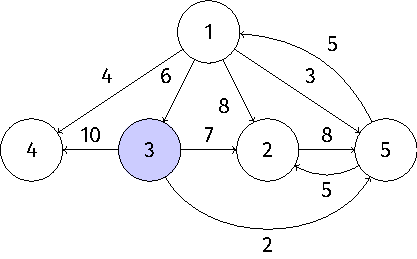
\includegraphics[center]{fig/8-2.pdf}
\end{frame}
\begin{frame}{计算过程}
    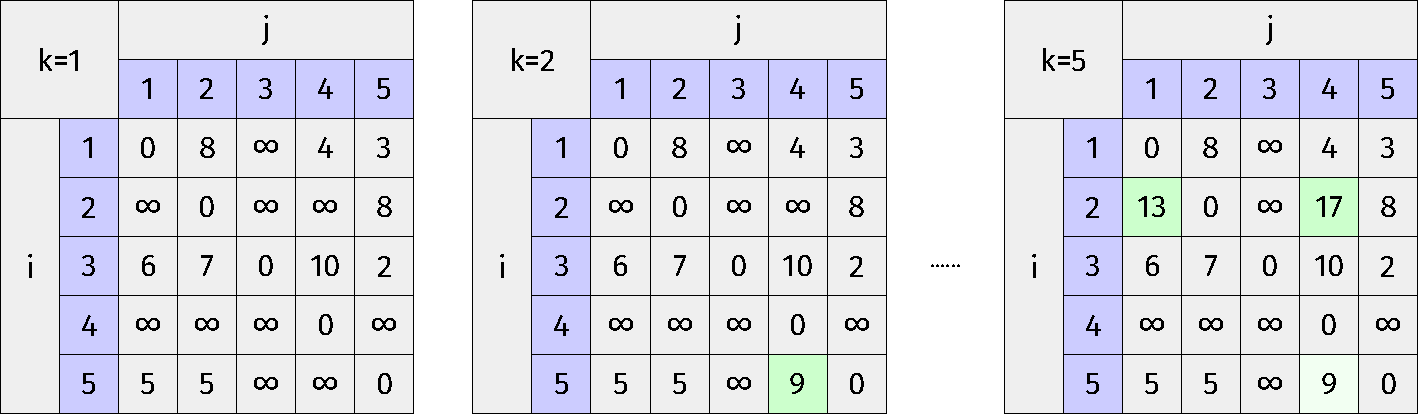
\includegraphics[scale=0.5,center]{fig/8-3.pdf}
    \begin{itemize}
        \item 上图显示了Floyd算法计算过程中的数组情况
        \begin{itemize}
            \item 其中$k=1$时是数组的初始情况
            \item $k=3,4$时数组内容没有发生变化
        \end{itemize}
        \item 最后在结果的邻接矩阵中,依次查找每个$i$到其他点$j$的距离的最大值,再从这些最大值中找到最小值,可以看到,最小的最大值为10,此时$i$为3
    \end{itemize}
\end{frame}
\begin{frame}{最短路径快速算法}
    \begin{itemize}
        \item \textcolor{blue}{贝尔曼-福特(Bellman–Ford)}算法:通过不停修改路径长度值$D$来达到求最短路径的目标,这种操作被称为\textcolor{blue}{松弛操作}。从$a$点到$b$点,不会超过$n-1$条边,第$i$次松弛操作,保证对距离源点$i$距离值最小,进行$n-1$次操作,就更新了到所有点的最短距离。该算法允许有负权边,并可以通过第$n$次操作检查$D$值变化情况来判断是否存在负权回路
        \vfill
        \item \textcolor{blue}{最短路径快速算法}(SPFA, Shortest Path Faster Algorithm)是对Bellman-Ford算法的优化,因为Bellman-Ford算法的松弛操作执行在所有的节点上,有很多节点并没有必要进行更新,SPFA算法通过队列维护备选节点,当节点被松弛后放入队列,直到没有终点被松弛。SPFA也适用于带有负边权的图,然而在最坏情况的时间复杂度与Bellman-Ford算法相同
\end{itemize}
\end{frame}
\begin{frame}{1511 -- Invitation Cards (poj.org)}
    \begin{itemize}
        \item $p$个公交站点,$q$条公交线路,从$u$站点到$v$站点,价格为$w$。$p$个志愿者从1号站点出发到每个站点,再返回到1号站点,求花费的总值最少是多少
        \vfill
        \item 处理一个点之后,将该点连接的路径放入队列,存储图信息的数据结构应该方便这个操作,可以使用\textcolor{blue}{邻接表}(Adjacency list)来实现,这里采用数组来模拟链表实现的邻接表(被称为\textcolor{blue}{链式前向星})\footnote{\url{https://malash.me/200910/linked-forward-star/}}
\end{itemize}
\end{frame}
\begin{frame}{链式前向星}
\begin{exampleblock}{Example}
\begin{columns}   
\column{0.3\textwidth}
\begin{table}
    \begin{tabular}{ccc}
        p  & q    \\\hline
        4  & 6    \\\hline
        u  & v  &  w   \\\hline
        1  & 2  & 10   \\\hline
        2  & 1  & 60   \\\hline
        1  & 3  & 20   \\\hline
        3  & 4  & 10   \\\hline
        2  & 4  & 5    \\\hline
        4  & 1  & 50   \\\hline
    \end{tabular}
\end{table}
\column{0.7\textwidth}
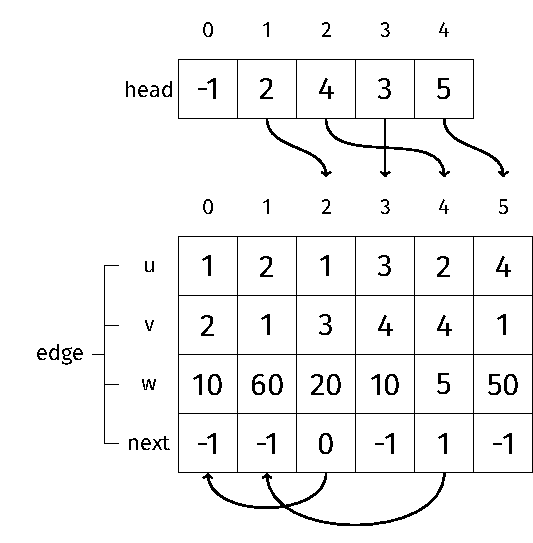
\includegraphics[scale=0.7]{fig/8-4.pdf}
\end{columns}
\end{exampleblock}
\end{frame}
\begin{frame}{1797 -- Heavy Transportation (poj.org)}
    \begin{itemize}
        \item $m$条街道有$n$个交点,交点编号从$1$到$n$,每条街道有重量限制$w$。从1号城市向$n$号城市运送起重机,选择一条路径,使得路径上的每条街道允许的重量$w$的最大值最大
        \item 如图,选择1-2-3,由于1-2允许的最大载重量为3,所以整条路线上允许的最大值是3;选择1-3,允许的最大值为4。最终结果为4
    \end{itemize}
    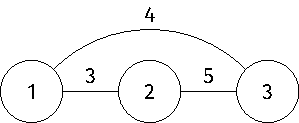
\includegraphics[center]{fig/8-5.pdf}
\end{frame}
\begin{frame}{Dijkstra算法}
    \begin{itemize}
        \item \textcolor{blue}{迪杰斯特拉(Dijkstra)}算法的特点是不断对两点间的最短距离$D$进行松弛操作
        \item S为源点,初始时令$D[S]=0$,其他$D$值设为无穷大,$T$为终点,$D[T]$为所求的最短路径,如果$D[T]$为无穷大,则不存在$S$到$T$的最短路径
        \item 具体操作过程是每次选择未访问的$D$值最小的一点$u$,将$u$标记为访问,再将与$u$连接的所有点$v$的$D[v]$的值更新为$D[v]$和$D[u]+a[u,v]$中的较小值
        \item Dijkstra算法比较之前的算法效率要高,但是不支持负权的边
        \item 分阶段松弛操作的本质是\textcolor{blue}{动态规划}
        \item Dijkstra算法的松弛操作针对的是累计从源点到目标点的最短距离值$D$,将$D$值的含义改为从源点到目标点的最大允许载重量,每次选择未访问的$D$值最大的一点$u$,更新$D[v]$为$D[v]$和$min(D[u],a[u,v])$的最大值,就是本题的解法
    \end{itemize}
\end{frame}
\begin{frame}{8.3 图的连通性}
    \begin{block}{连通图}
        如果图中任意两点都是连通的,那么图被称作连通图
    \end{block}
    \vfill
    \begin{block}{强连通分量(Strongly connected component)}
        图的一个子图,里面的所有点构成一个强连通图, 即每一个顶点都可以通过图中的边到达图中其他的顶点,且这个连通子图是极大的,也就是子图外不再包含符合该条件的点
    \end{block}
    \vfill
    \begin{itemize}
        \item 在图的规模较小时,可以模仿Floyd算法对所有边进行枚举,但是深入理解\textcolor{blue}{Tarjan算法},了解low和dfn的含义,能够更有效的解决图的连通性问题
    \end{itemize}
\end{frame}
\begin{frame}{Tarjan算法}
    \begin{itemize}
        \item 图中每个节点的两个数字分别是执行了Tarjan算法后的dfn值和low值,该图最终被划分出了4个强连通分量
    \end{itemize}
    \vfill
    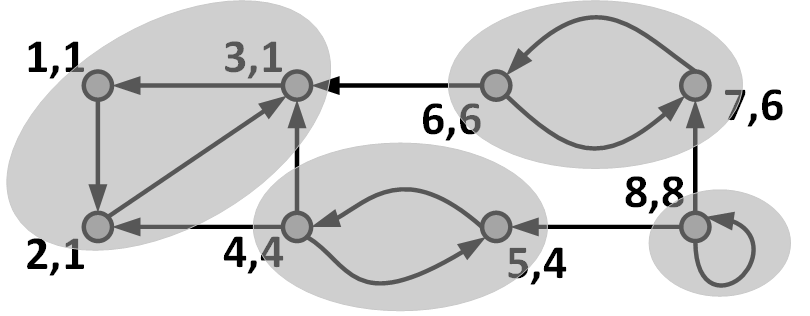
\includegraphics[width=0.5\textwidth,center]{fig/tarjan.png}
    \scriptsize{
    \begin{enumerate}[(1)]
        \item 从图中一点$u$出发,对图进行深度优先搜索,用dfn[u]记录节点u在深度优先搜索中访问的次序编号,low[u]记录$u$或$u$的子树能够追溯到的最早的栈中节点的次序编号。将$u$放入堆栈,搜索$u$的相连点$v$,如果$v$未被访问,则递归访问$v$;如果$v$已经在堆栈中,则检查dfn[v]是否小于low[u],如果是,就更新low[u]的值为dfn[v]
        \item 用U[i]表示u属于哪个强连通分量,按照深度优先搜索规则,同一强连通分量的节点会依次入栈,当发现dfn[u]等于low[u],说明搜索回到了强连通分量的最初搜索点,此时依次将这些low值相同的点出栈,将它们的U值设置成同一个编号
        \item 对图中所有点重复1,2操作,这样每个的强连通分量就缩成了对应的U[i]点
    \end{enumerate}}
\end{frame}
\begin{frame}{2186 -- Popular Cows (poj.org)}
    \begin{itemize}
        \item 有$n$头牛,$m$对关系,关系$(a,b)$表示$a$认为$b$是受欢迎的,这种关系是可传递的,即$(a,b)(b,c)$可以推出$(a,c)$,现在找出被所有其他牛都认为受欢迎的牛的数量
        \item 将$a,b$看作图中的节点,关系$(a,b)$看成点$a$到点$b$的一条有向边,题目所求的相当于找到这样点,所有的点都可以找到一条路径通向该点
        \begin{itemize}
            \item 把图进行简化,确定图中的强连通分量,我们发现,问题中强连通分量中的点对外具有相同的性质,可以将它们当成一个点来对待,如果其中一点符合题解,则强连通分量中所有点都符合题解
            \item 通过Tarjan算法,找到的强连通分量都缩成一点U[i],接下来,在由U点组成的有向无环图中检查各个节点的出度。由于消除了环路,所以一定存在出度为0的点。如果存在唯一的出度为0的点,则这个点就是题目要求的点,该点所在的强连通分量里点的数量就是题解
        \end{itemize}
    \end{itemize}
\end{frame}
\begin{frame}{1144 -- Network (poj.org)}
    \begin{itemize}
        \item 电话网络有$n$个连接点$1$到$n$,每个连接点有一个交换机,两个交换机之间的路线双向的。如果交换机停机会造成某些点不能连通,这个交换机称为关键节点,求所有关键节点的数量
        \begin{exampleblock}{例(红色为关键节点)}
            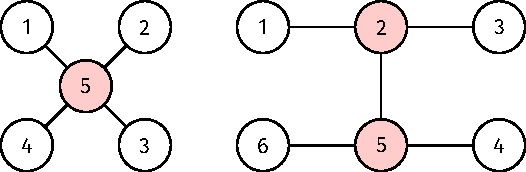
\includegraphics[scale=.8,center]{fig/8-6.pdf}
        \end{exampleblock}
        \item 在无向的连通图中,删除一点后使图不再连通,这点就被称为\textcolor{blue}{割点}(vertex separator/vertex cut)
        \item 与割点类似,如果删除一条边使图不再连通,这条边被称为\textcolor{blue}{桥}(Bridge)
        \item 求割点的数量,采用\textcolor{blue}{Tarjan的找桥算法}来实现
    \end{itemize}
\end{frame}
\begin{frame}{Tarjan找桥算法}
    \begin{itemize}
        \item 与有向图求强连通分量的算法类似,对连通图采用深度优先搜索,通过标记dfn和low的值来进行判断,不同之处有以下几点:
        \begin{enumerate}[(1)]
            \item 不需要使用堆栈对节点进行分类
            \item 无需对每个节点都进行一次深度优先搜索,选中一点作为起始节点即可
            \item 因为无向图的边是双向的,在找$u$点的后序节点时,需要避免访问$u$的父亲节点
            \item 对起始节点需要特殊判断,如果遍历过程中它的子节点超过1个,则它也是一个割点,如上图右图,1位置为起始节点的话不是割点,而2位置为起始节点,它的子节点有3个,所以它是割点
        \end{enumerate}
        \item low[v]≥dfn[u]时说明v点能够追溯到的最早节点编号是$u$点或者$u$点之后,所以$u$为割点;如果改成low[v]>dfn[u],说明$v$点能够追溯到的最早节点编号在$u$点之后,意味着去掉边$(u,v)$后图不再连通,$(u,v)$就是一个桥
    \end{itemize}
\end{frame}
\begin{frame}{8.4 网络流问题}
    \begin{block}{网络流}
        在图论中,网络流(Network flow)是指在一个每条边都有容量(Capacity)的有向图分配流,每条边的流量不会超过它的容量
    \end{block}
    \vfill
    \begin{itemize}
        \item 通常在运筹学中,有向图称为网络。顶点称为\textcolor{blue}{节点}(Node)而边称为\textcolor{blue}{弧}(Arc)
        \item 一道流必须符合一个结点的进出的流量相同的限制, 除非是:
        \begin{itemize}
            \item \textcolor{blue}{源点}(Source):有较多向外的流
            \item 或是\textcolor{blue}{汇点}(Sink):有较多向内的流
        \end{itemize}
        \item 一个网络可以用来模拟道路系统的交通量、管中的液体、电路中的电流或类似一些东西在一个结点的网络中游动的任何事物
    \end{itemize}
\end{frame}
\begin{frame}{8.5 二分图问题}
    \begin{block}{二分图}
        一个图所有节点可以分为两个独立的集合$U,V$,所有边分别连接两个集合中的一个点,这样就构成了一个二分图(Bipartite graph)
    \end{block}
    \begin{itemize}
        \item 二分图匹配是一类特殊形式的网络流问题,通过构图,利用二分图最大匹配算法,可以解决图算法中一些问题,例如:
        \vfill
        \begin{itemize}
            \item \textcolor{blue}{最小顶点覆盖}(最小顶点覆盖数=二分图最大匹配的边数)
            \item \textcolor{blue}{最大独立集}(最大独立集点数=总点数-二分图最大匹配边数)
            \item \textcolor{blue}{DAG图最小可相交路径覆盖}(DAG图最小可相交路径覆盖数=总点数-二分图最大匹配边数)
        \end{itemize} 
    \end{itemize}
\end{frame}
\begin{frame}{匈牙利算法}
    \begin{itemize}
        \item 匈牙利算法 ,也称KM(Kuhn–Munkres)算法,是寻找最大匹配的经典算法, 主要思想是:
        \begin{itemize}
            \item 在已有匹配的情况下,$U$中取未配对的一点$i$,找它连向$V$的边$(i,j)$,如果$j$没有和其他点配对,则将$j$分配给$i$,匹配边数加1
            \item 如果$j$已经和$U$中$k$配对,就对$j$进行递归操作,将$k$换掉,将$j$分配给$i$
            \item 如果可以成功,匹配边数加1,直到所有点都结束匹配
        \end{itemize}
        \vfill
        \item 匹配过程就是网络流问题中找增广路径的过程,每次更新过程称为一次\textcolor{blue}{增广}
    \end{itemize}
\end{frame}
\begin{frame}{2239 -- Selecting Courses (poj.org)}
    \begin{itemize}
        \item 大学有$n$门课,每门课重复$t$次,每次在每周的第$p$天的第$q$时间段上课,求在不冲突的情况下,每周最多可以选多少门课
        \item 分析:
        \begin{itemize}
            \item 每周7天,每天12个时间段,共有84个时间段,对应84个节点,增加一个源点$s$连接每个节点,边容量为1,增加一个汇点$t$,每个节点到汇点的容量为1,这样,从$s$到$t$的最大流就是最多可以上课的总数
            \item 在不添加源点和汇点的情况下,$n$门课对应$n$个节点,作为集合$U$,84个时间段作为另一个集合$V$,从$U$集合中的节点到$V$集合中的节点,如果某门课在某个时间段上课,就存在一条边,这就构成了一个二分图
            \item 一个图中,如果其子图中每两条边都没有公共端点,这个子图叫做一个\textcolor{blue}{匹配}(Matching),边数最多的匹配称为\textcolor{blue}{最大匹配}(maximal matching),这个题也可以看成求二分图中的最大匹配问题
        \end{itemize}
    \end{itemize}
\end{frame}
\end{document}